\section{Transform}

In order to explain our algorithm consider the following notation: $i$ refers to the $i-th$ frame in the original video, and $i'$ refers to the $i-th$ frame in the stabilized video.

Initially, we considered the following algorithm to compute $i'$:
\begin{enumerate}
	\item extract keypoints($X$) from $(i-1)'$
	\item extract keypoints($Y$) from $i$
	\item find matches($M$) between $X$ and $Y$
	\item compute transformation $T$ from $M$.
	\item apply transformation $T$ to $i$
\end{enumerate}

With this approach, we were obtaining a lot of misstransformations(Figure xxx) because the difference between $i$ and $(i-1)'$ are complex. Thus we defined anothe approach:   

\begin{enumerate}
	\item extract keypoints($X$) from $i-1$
	\item transform keypoints location of $i-1$ based on $(i-1)'$
	\item extract keypoints($Y$) from $i$
	\item find matches($M$) between $X$ and $Y$
	\item compute transformation $T$ from $M$.
	\item apply transformation $T$ to $i$
\end{enumerate}

We assume that the difference between adjacent frame in the original video is small. Thus, we compare the feature vector of $i$ and $i-1$, but the keypoints location of $i$ and $(i-1)'$.

Once we have the transformation of parameters we apply it for every pixel in $i$, depending of the movement, some black holes and lines appears(Figure \ref{fig:diff-interpolation}). Thus, we interpolate this points with the average of four neighbors and fill with zero the cases when the neighbors are also empty.

\begin{figure}[!h]
	\centering
	\begin{subfigure}{0.5\textwidth}
	  \centering
	  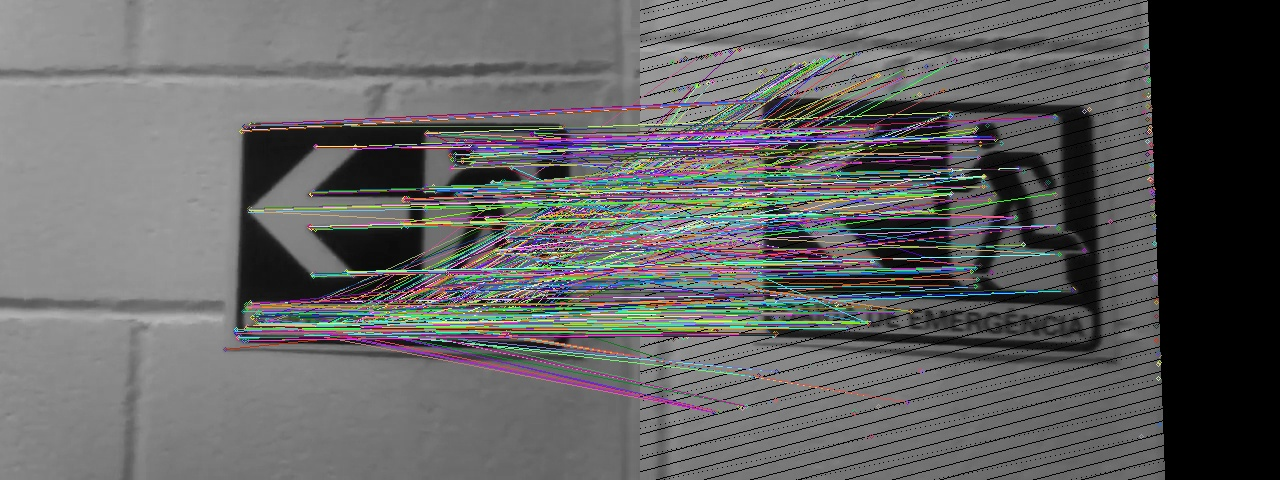
\includegraphics[width=0.8\linewidth]{figs/without-interpolation.jpg}
	  \caption{Without interpolation}
	\end{subfigure}%
	\begin{subfigure}{0.5\textwidth}
	  \centering
	  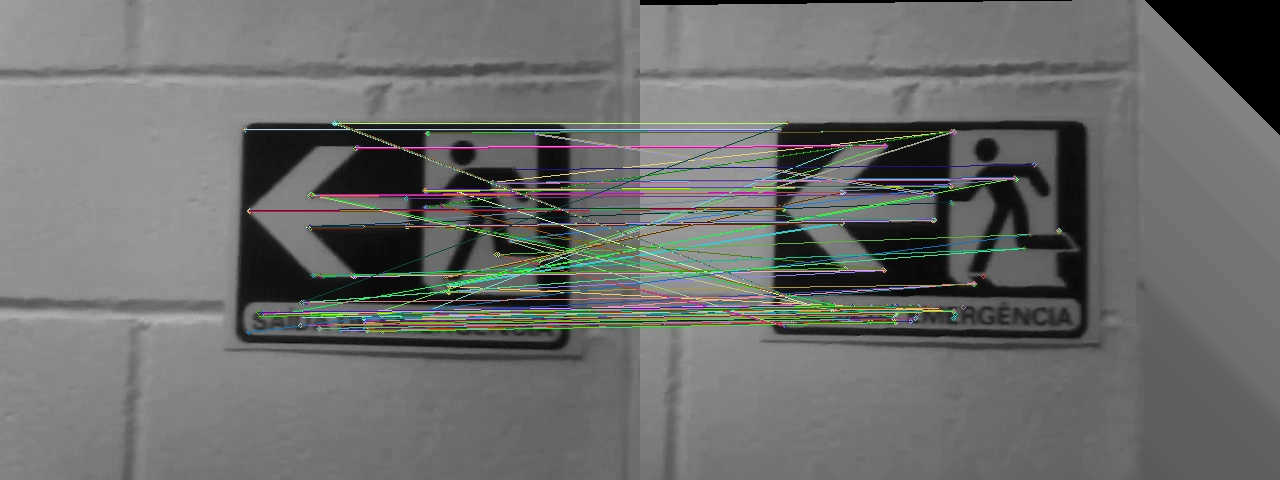
\includegraphics[width=0.8\linewidth]{figs/with-interpolation.jpg}
	  \caption{With interpolation}
	\end{subfigure}%
	 \caption{Comparison of results fof transformation uisng interpolation}
	\label{fig:diff-interpolation}
\end{figure}



